\section{问题一：数据质量与领域配比}
\label{sec:q1}

问题一解决语料质量的量化评价与训练领域配比选择问题。本章依次完成三件事：建立可复现的文档及领域质量分，诊断评价指标之间的分歧，并在实验覆盖范围内建立配比与验证损失的关系、选出推荐配比。所得领域质量 $Q_i$、推荐配比 $\bp^*$、配比—损失关系与尺度校准信息经 P1 接口传入问题二，为广义标度律中的质量项和配比项提供输入，并为问题三的资源配置和问题四的检验预测提供基础。

\subsection{任务一：数据质量评价}
\label{sec:q1_task1}

预训练语料的质量影响模型从数据中获取的信息，也是后续领域配比建模的重要输入。然而，语料质量缺少统一定义和人工标注真值，现有自动评价字段又存在形态、尺度与方向差异。A1 包含七个领域的 51,230 篇文档，用于确定质量评价方法及全部参数；A2 的 17,523 篇 arxiv 文档和 A3 的 203,752 篇 github 文档作为扩展集，在参数冻结后接受同一套评分，并用于检查评分分布的稳定性。

因此，任务一的本质是无人工真值条件下的多指标综合评价。我们先处理字段形态、评价方向、量纲和长度混杂，将原始字段转为可比指标；再依据指标的信息量及相关性确定权重，稳健合成为文档质量分，并汇总得到领域质量。以下依次说明数据预处理和综合评价模型。

\subsubsection{数据预处理}
\label{sec:q1_preproc}

数据预处理把 A1 的 22 个原始字段整理成 25 项方向一致、取值于 $[0,1]$ 的可比指标。原始字段的输出形式不同，不能直接拼接或比较：四项 \texttt{modernbert\_*} 各输出六档 logits，取 softmax 后的期望分；\texttt{qurater} 的四维向量拆成四项指标，是 22 项展开为 25 项的唯一来源；\texttt{ad\_en} 与 \texttt{fluency\_en} 取标签 1 的预测概率，其中前者的标签 1 表示「无广告」；\texttt{fineweb\_edu} 从单元素向量中取标量值。

11 项 \texttt{rps\_*} 是规则型文本统计，其中词数、句数、平均词长和词熵四项不宜简单按「越高越好」处理，故以各域 A1 中位数为适宜中心，将偏离程度转为负值；其余指标按含义统一正负方向，对适用的重尾非负量作 $\log(1+x)$ 变换。这样既保留规则统计的信息，又避免把极端长度或熵值直接解释为更高质量。

DSIR 的三项重采样权重还存在明显的长度混杂。未经处理时，它们与词数的 Spearman 相关在 A1 七域中均为负，21 组「领域—指标」的绝对相关中位数达 $0.957$：若直接纳入评分，文档长短可能被误当成质量差异，影响文档排序和领域汇总。为削弱这一关系，先将 DSIR 除以 $\max(\text{词数},1)$，再在 A1 各域内对 $\log(1+\text{词数})$ 回归并取残差；A2/A3 复用 A1 的回归系数。

图~\ref{fig:F2_dsir_length_correction} 把同一「领域—指标」在原始、除词数、残差化三个阶段的词数绝对相关连成一条线。中位数在除词数后降至 $0.599$，残差化后降至 $0.095$，说明长度关联明显减弱，但并未完全消失；book 域最高剩余 $|\rho|=0.503$，该域仍需谨慎解释。相关降低只表明长度影响减少，不能据此断言指标更接近真实质量。

\begin{figure}[H]
\centering
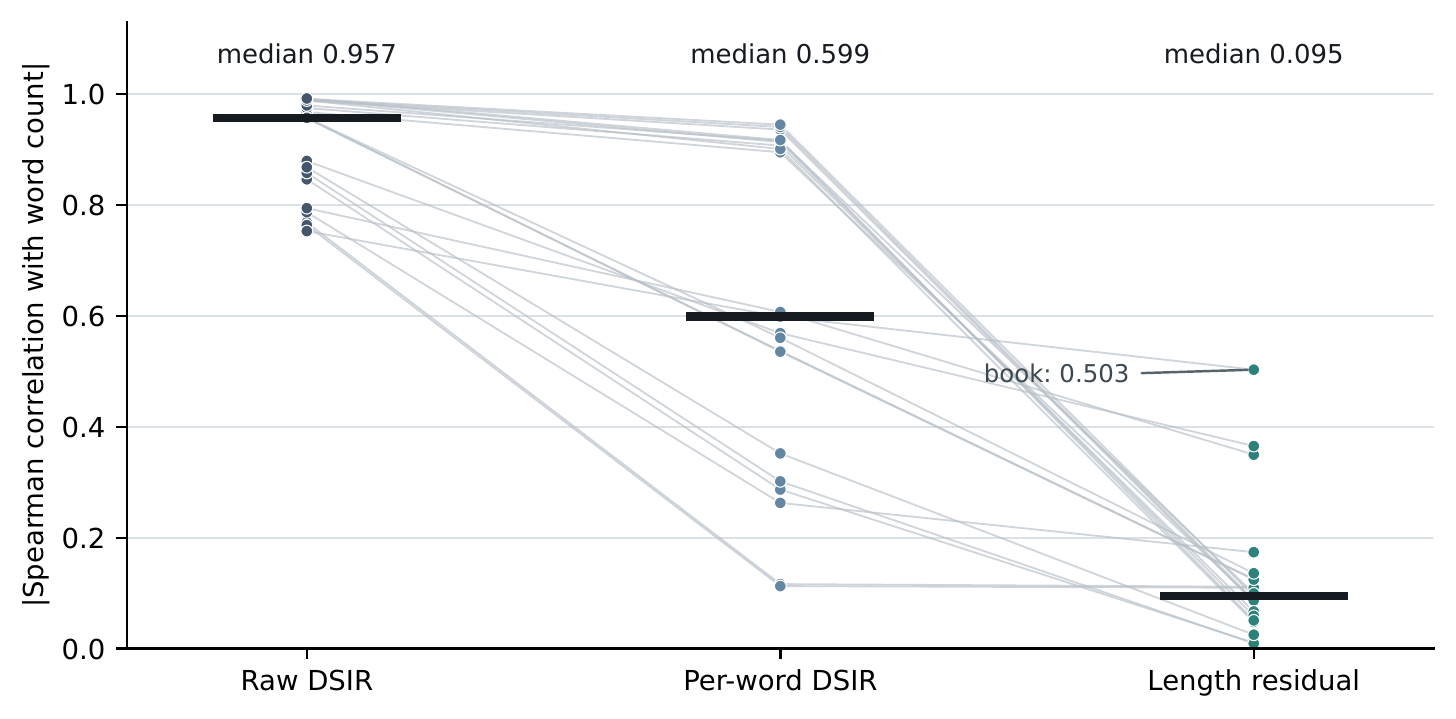
\includegraphics[width=0.88\textwidth]{figs/q1_F2_dsir_length_correction.png}
\caption{A1 七域三项 DSIR 指标在长度校正前后的词数绝对 Spearman 相关（每条细线对应一组领域—指标，黑线为 21 组中位数）}
\label{fig:F2_dsir_length_correction}
\end{figure}

最后，各域各指标用 A1 的 $1\%/99\%$ 分位缩尾，按 A1 端点 Min–Max 归一到 $z_j(x)\in[0,1]$，缺失值用 A1 同域同指标的标准化中位数填补。回归系数、适宜中心、缩尾分位、归一端点和填补值均只在 A1 上确定并冻结，A2/A3 仅作前向应用，使三集分数遵循同一评价规则。

\subsubsection{数据质量综合评价模型}
\label{sec:q1_quality_model}

预处理后得到 25 项可比指标，首先要确定各项指标的权重。表~\ref{tab:q1_weight_methods} 比较了三种常用赋权方法在本题无人工质量真值、多项指标同源的条件下各自能解决的问题与局限。

\begin{table}[H]
\centering\small
\caption{质量指标赋权方法在本题条件下的比较}
\label{tab:q1_weight_methods}
\begin{tabularx}{\textwidth}{@{}p{2.0cm} X X@{}}
\toprule
方法 & 优点 & 在本题中的局限 \\
\midrule
层次分析法 & 可表达专家对不同质量维度的判断 & 缺少人工质量标注与稳定的专家判断依据，权重难以复现 \\
熵权法 & 由指标离散程度客观定权，无需人工标注 & 同源且高度相关的指标可能因各自离散而被重复计权 \\
CRITIC & 同时考虑指标离散程度与指标间相关性，可减轻冗余计权 & 依据总体相关结构定权，不能单独处理某篇文档的极端或对立指标 \\
\bottomrule
\end{tabularx}
\end{table}

本题需要一套只由 A1 确定、可冻结并应用于 A2/A3 的权重。CRITIC 方法\cite{critic} 同时利用指标的区分能力和相关结构，适合抑制同源指标的重复贡献，因此采用它计算固定权重：
\begin{equation}
\label{eq:q1_critic}
C_j=s_j\sum_{k=1}^{25}(1-r_{jk}),\qquad w_j=\frac{C_j}{\sum_k C_k},\qquad \sum_j w_j=1 .
\end{equation}
其中 $s_j$ 为 A1 标准化指标的样本标准差，$r_{jk}$ 为指标 $j,k$ 的 Pearson 相关系数。赋权解决的是总体冗余，逐篇合成仍要面对另一现象：部分指标远离同篇其余指标，低端极值若直接进入算术均值，可能把局部异常意见放大为整篇文档的低质量分；同一来源组内部也可能出现相反意见，下一任务将专门诊断这种冲突。普通中位数虽能削弱极值，却不利用权重和偏离幅度。因此本文用加权 Huber 中心\cite{huber} 合成文档分数：在中心附近保留加权平方损失，对超过阈值 $\delta$ 的偏离限制边际影响，从而减弱单项极端指标拉低综合分的作用。
\begin{equation}
\label{eq:q1_huber}
Q(x)=\arg\min_{q\in[0,1]}\sum_{j=1}^{25}w_j\rho_\delta\bigl(z_j(x)-q\bigr),\qquad
\rho_\delta(u)=\begin{cases}\tfrac12u^2,&|u|\le\delta,\\ \delta(|u|-\tfrac12\delta),&|u|>\delta,\end{cases}
\end{equation}
由方程 $\sum_j w_j\operatorname{clip}(q-z_j,-\delta,\delta)=0$ 在 $[0,1]$ 上二分求解。阈值 $\delta$ 仅由 A1 确定：取每篇的加权指标中位数 $m_x$ 与加权 MAD $a_x=\operatorname{wmedian}_j|z_j-m_x|$，再令 $\delta=1.345\times1.4826\times\operatorname{median}_{x\in A1}a_x\approx0.4035$（$1.4826$ 为正态尺度校正、$1.345$ 为 Huber 经典效率常数）。25 项权重介于 \texttt{fineweb\_edu} $0.0359$ 与 \texttt{modernbert\_professionalism} $0.0671$ 之间，没有任何单一指标主导评分。综合质量分确定后，任务二再按来源追查组内与组间的相反意见；该诊断不反向调整本式的权重或分数。

\subsubsection{领域质量结果与稳健性检验}
\label{sec:q1_domain_quality}

\paragraph{领域质量结果}领域质量取域内文档分数的中位数，并以 2,000 次文档 bootstrap 给出条件 $95\%$ 区间。表~\ref{tab:q1_domain_quality} 同时列出 A1 七域、A2 的 arxiv 与 A3 的 github；扩展集只与 A1 的同名领域比较。

\begin{table}[H]
\centering\small
\caption{A1 抽样集与 A2/A3 扩展集的领域综合质量分（数据源：\texttt{T2\_domain\_quality.csv}）}
\label{tab:q1_domain_quality}
\begin{tabularx}{\textwidth}{@{}l l r r X r@{}}
\toprule
数据集 & 领域 & 文档数 & 中位数 $Q$ & bootstrap $95\%$ 区间 & 相对 A1 同域差值 \\
\midrule
A1 & arxiv & 1,419 & 0.7707 & $[0.7671,0.7754]$ & --- \\
A2 & arxiv & 17,523 & 0.7697 & $[0.7688,0.7705]$ & $-0.0010$ \\
A1 & commoncrawl & 9,640 & 0.6761 & $[0.6739,0.6784]$ & --- \\
A1 & stackexchange & 10,000 & 0.6600 & $[0.6582,0.6621]$ & --- \\
A1 & c4 & 10,000 & 0.6545 & $[0.6525,0.6566]$ & --- \\
A1 & book & 171 & 0.6313 & $[0.6138,0.6500]$ & --- \\
A1 & github & 10,000 & 0.6172 & $[0.6157,0.6189]$ & --- \\
A3 & github & 203,752 & 0.6158 & $[0.6154,0.6162]$ & $-0.0014$ \\
A1 & wikipedia & 10,000 & 0.5991 & $[0.5971,0.6015]$ & --- \\
\bottomrule
\end{tabularx}
\end{table}

A1 中 arxiv 的中位质量最高，wikipedia 最低；图~\ref{fig:F2_domain_quality_box} 展示了七域的完整分布，说明只看一个域级点估计仍会遗漏域内变异。

\begin{figure}[H]
\centering
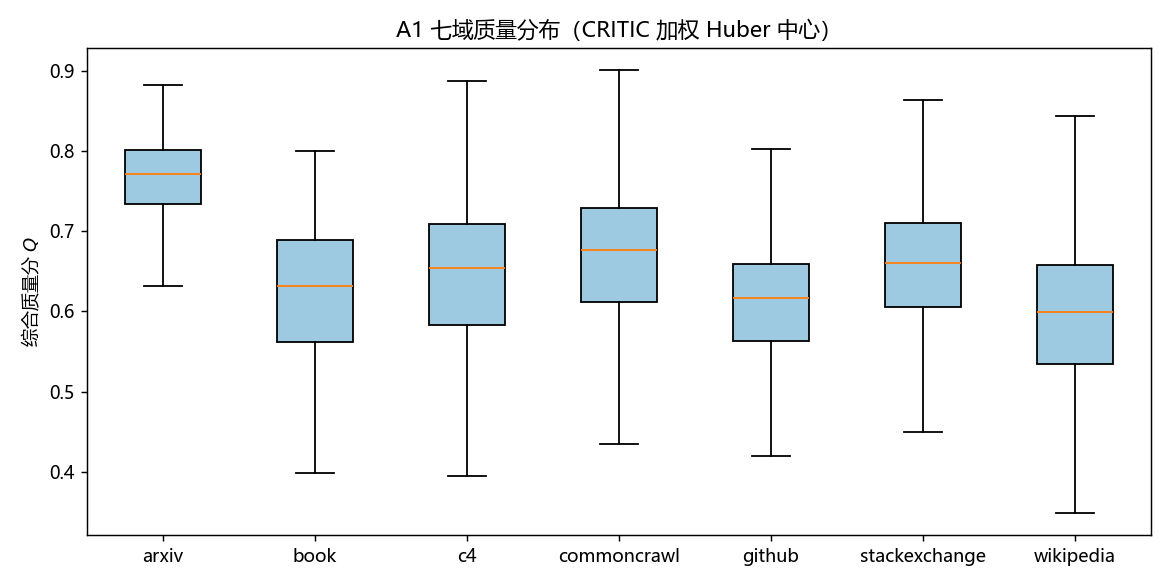
\includegraphics[width=\textwidth]{figs/q1_F2_domain_quality_box.png}
\caption{A1 七域的 CRITIC 加权 Huber 综合质量分分布}
\label{fig:F2_domain_quality_box}
\end{figure}

\paragraph{抽样集与扩展集对照}A2 arxiv 与 A1 同域中位数相差 $-0.0010$，A3 github 与 A1 同域相差 $-0.0014$；两组分布的 KS 距离分别为 $0.0265$、$0.0107$。这表明在相同评分规则下，两域抽样结果与扩展集接近。A1 的对应文档包含在 A2/A3 中，因此该对照检查的是抽样代表性，不能当作独立质量真值验证。

\paragraph{稳健性核验}综合质量分与同权重算术均值、PCA、TOPSIS 的文档排序 Spearman 分别为 $0.9936$、$0.8166$、$0.9588$：它与算术均值的排序几乎一致，PCA 对部分文档的排序则有明显调整，不能说合成方法完全不影响结果。逐篇剔除最偏离的一个指标后，在极端程度最高 $10\%$ 的文档（5,123 篇）中，综合质量分的绝对变动中位数为 $0.0260$（P90 $0.0340$），算术均值为 $0.0374$（P90 $0.0488$）。这些数值是 $[0,1]$ 评分尺度上的变动，说明 Huber 中心对单项极端意见约少受 $30\%$ 影响，不说明它更接近未知的真实质量。

由于没有人工质量真值，本任务只能报告方法一致性与扰动稳健性，不能报告质量准确率；这一证据边界在后文模型评价部分继续讨论。

\subsection{任务二：质量冲突消解}
\label{sec:q1_task2}

任务一发现，同一文档的质量指标可能给出相反评价，甚至同组指标也会分裂。这类分歧并不修改任务一得到的综合质量分，而是需要被识别出来并解释其来源，以判断单个质量分是否可靠、哪些文档值得优先复核。为此，本任务先在 \ref{sec:q1_conflict_def} 定义冲突及筛查阈值，再在 \ref{sec:q1_conflict_types} 划分类型并分析可能成因，最后比较折扣处理前后的质量分。

\subsubsection{质量冲突的定义与识别}
\label{sec:q1_conflict_def}

这里的质量冲突，指同一文档的指标在各自参照分布中处于明显相反的位置，而非文档质量已被证实有误。原始分数的量纲不同，不能直接相减。我们先按生成机制把 25 项指标分为 RPS（11 项）、DSIR（3 项）、轻量分类器（2 项，即 \texttt{ad\_en} 与 \texttt{fluency\_en}）、FineWeb-Edu（1 项）\cite{fineweb}、QuRating（4 项）和 ModernBERT（4 项）；每项只归入一个来源，避免指标多的来源在比较中自然占优。

对领域 $d$ 的指标 $j$，用 A1 同域经验分布将标准化分 $z_j(x)$ 转为百分位排名 $r_j(x)=F_{dj}^{A1,\mathrm{mid}}(z_j(x))$，同值取中秩。再取来源 $s$ 内指标排名的中位数 $m_s(x)$，并按 A1 同域的来源中心分布将其转为 $u_s(x)$；A2/A3 沿用 A1 的参照分布。这样六个来源各提供一个可比的相对评价，来源间冲突程度定义为
\begin{equation}
\label{eq:q1_B}
B(x)=\max_{s=1,\dots,6}u_s(x)-\min_{s=1,\dots,6}u_s(x).
\end{equation}

\(B(x)\) 越大，最高与最低来源的相对评价相距越远。以 A1 各域 $B$ 的第 95 百分位为阈值 \(\tau_d\)，将 \(B(x)>\tau_d\) 的文档列为高分歧候选；A2/A3 使用相应 A1 域的同一阈值。P95 将 A1 每域的候选比例控制在约 $5\%$，这是预设筛查范围，不是真实冲突率。图~\ref{fig:F3_threshold_sensitivity} 比较 P90、P95、P97.5 三档：A1 候选比例依次约为 $10.00\%$、$5.00\%$、$2.50\%$，A2 为 $9.19\%$、$4.73\%$、$2.00\%$，A3 为 $9.74\%$、$4.99\%$、$2.44\%$。阈值越严格，入选文档越少；三集变化方向一致，但这不能证明哪档阈值更准确。

\begin{figure}[H]
\centering
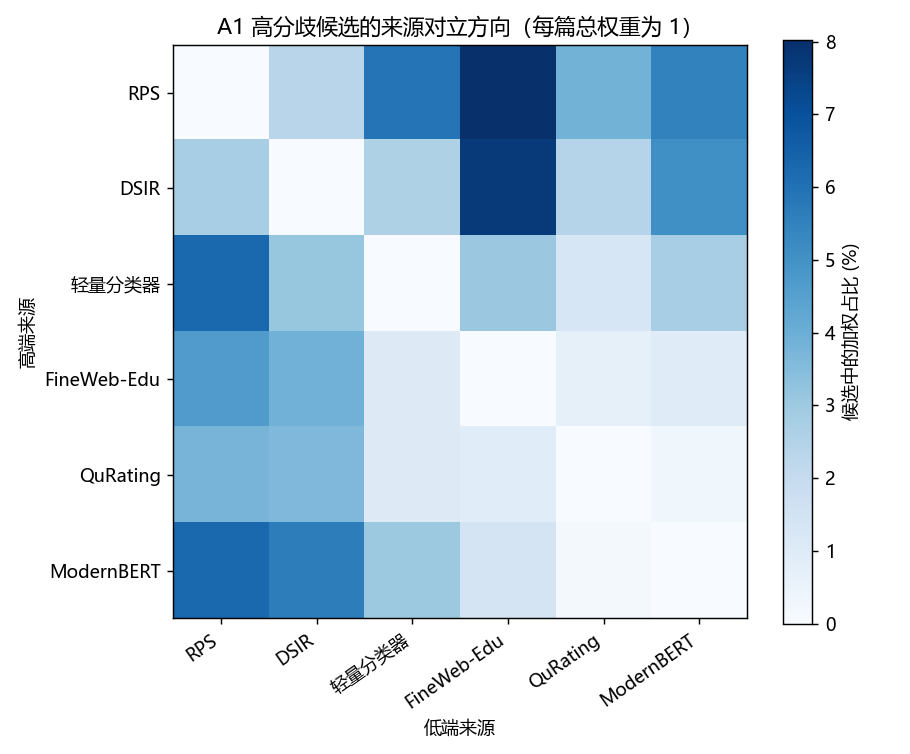
\includegraphics[width=\textwidth]{figs/q1_F3_threshold_sensitivity.png}
\caption{A1 阈值分位变化对 A1–A3 高分歧候选比例的影响}
\label{fig:F3_threshold_sensitivity}
\end{figure}

\subsubsection{冲突类型以及成因分析}
\label{sec:q1_conflict_types}

\ref{sec:q1_conflict_def} 已圈定高分歧文档，但还需分清分歧由多少来源支持。若高端 \(u_s\ge0.8\) 与低端 \(u_s\le0.2\) 各有至少两个来源，记为「多来源对立」；其余高分歧文档记为「稀疏来源对立」。另用来源内跨度和逐指标留一偏离，单列未达到来源间高分歧、仅一个指标在一个来源中明显偏离的「单指标独有」候选。前两类共同划分高分歧集合，第三类属于另一套筛查口径，不与前两类相加。

表~\ref{tab:q1conflict} 显示，A1 的 2,561 篇高分歧文档中，695 篇达到多来源对立条件，其余 1,866 篇属于稀疏来源对立。A2/A3 的高分歧比例接近 A1，分别为 $4.73\%$ 与 $4.99\%$；这表明筛查工作量在扩展集上相近，不能解释为真实质量错误的比例。

\begin{table}[H]
\centering\small
\caption{A1–A3 质量冲突候选的类型与规模（数据源：\texttt{T3\_six\_source\_candidate\_summary.csv}）}
\label{tab:q1conflict}
\begin{tabularx}{\textwidth}{@{}lccc@{}}
\toprule
候选类型 & A1：51,230 篇 & A2：17,523 篇 & A3：203,752 篇 \\
\midrule
来源间高分歧 & 2,561（5.00\%） & 829（4.73\%） & 10,167（4.99\%） \\
其中多来源对立 & 695（1.36\%） & 277（1.58\%） & 3,598（1.77\%） \\
其中稀疏来源对立 & 1,866（3.64\%） & 552（3.15\%） & 6,569（3.22\%） \\
单指标独有 & 2,879（5.62\%） & 709（4.05\%） & 8,606（4.22\%） \\
\bottomrule
\end{tabularx}
\end{table}

来源内部的不一致是第一种可能成因。图~\ref{fig:F3_source_internal} 以组内指标排名的 P90--P10 跨度比较六个来源：A1 的 RPS 跨度中位数为 $0.625$，远高于 DSIR 的 $0.037$；两组的 Kendall $W$ 分别为 $0.140$ 和 $0.967$。RPS 同时包含长度、重复和符号等不同侧面的规则统计，因而组内意见更容易分散；FineWeb-Edu 只有一项指标，内部跨度不定义。

\begin{figure}[H]
\centering
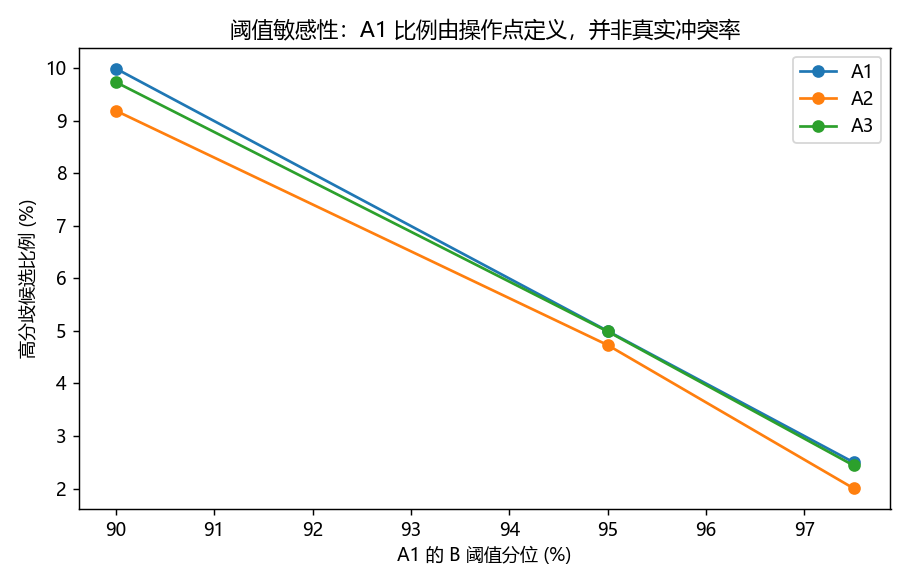
\includegraphics[width=\textwidth]{figs/q1_F3_source_internal.png}
\caption{A1 六来源内部跨度与一致性对照}
\label{fig:F3_source_internal}
\end{figure}

A1 有 $69.45\%$ 的文档在 RPS 内同时出现低于 $20\%$ 和高于 $80\%$ 的指标排名，说明将 11 项规则统计压成一个来源中位数会遮住组内分歧；这些相反排名并不等于某项指标测量错误。

第二种可能成因是不同评价机制关注的质量侧面不同。图~\ref{fig:F3_source_opposition} 的纵轴为高评价来源、横轴为低评价来源，每篇高分歧文档的来源配对总权重为 1；A1 最常见的是「RPS 高、FineWeb-Edu 低」，占高分歧候选的 $8.03\%$。A3 的同方向份额为 $13.03\%$，A2 则以「ModernBERT 高、FineWeb-Edu 低」最高（$9.89\%$）。主导方向随语料域变化，提示规则统计与模型评分器侧重不同，但没有人工真值，不能据此判定哪一方正确。

\begin{figure}[H]
\centering
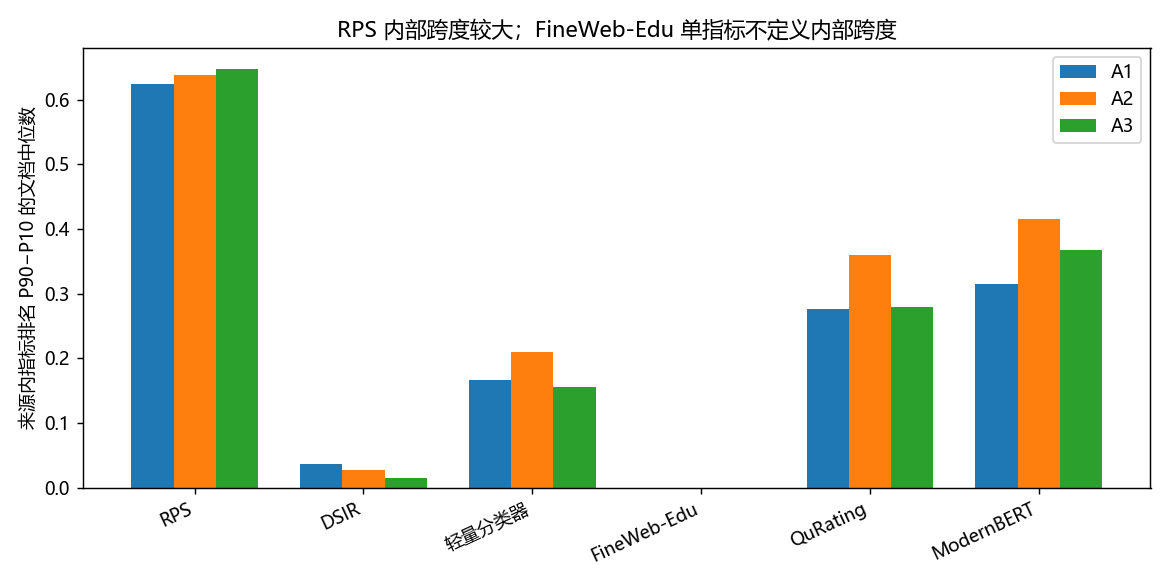
\includegraphics[width=\textwidth]{figs/q1_F3_source_opposition.png}
\caption{六来源对立方向的加权份额}
\label{fig:F3_source_opposition}
\end{figure}

与历史四组法比较时，原阈值选出的 A1/A2/A3 候选比例为 $19.08\%/24.52\%/23.28\%$，明显高于六来源约 $5\%$；直接比较两法会把阈值差异也算进去。按 A1 各域前 $5\%$ 对齐筛查比例后，两法在三集上的 Jaccard 为 $0.324/0.283/0.259$，说明即使入选规模相近，来源划分和排名方式仍会改变候选集合；重合度不能当作识别准确率。

\subsubsection{折扣对照模型 $Q_{\rm v2}$}
\label{sec:q1_qv2}

为检验来源内部一致性对综合分的影响，本文另建一个折扣对照模型。其数学形式借鉴 Dempster–Shafer 证据理论中的可靠性折扣\cite{shafer}：将每个来源的指标意见视为证据，以该来源的 Kendall $W$ 作为折扣系数，对原 CRITIC 权重作折扣后再归一化合成：
\begin{equation}
\label{eq:q1_wv2}
\tilde w_j=\frac{w_j\,W_{s(j)}}{\sum_k w_k\,W_{s(k)}},\qquad Q_{\rm v2}(x)=\arg\min_q\sum_j\tilde w_j\,\rho_\delta\bigl(z_j(x)-q\bigr).
\end{equation}
$Q_{\rm v2}$ 与综合质量分在 A1/A2/A3 的全局 Spearman 为 $0.9547/0.9207/0.9395$，A1 七域中位数排序未变，但分数水平有所调整，例如 arxiv 上升 $0.0303$、wikipedia 下降 $0.0583$。A1 高分歧候选与其余文档的 $Q_{\rm v2}-Q$ 中位数分别为 $-0.0260$、$-0.0309$，变化并未集中在候选文档上。因此该折扣模型只用于检查来源权重改变的影响，不能称为已验证的冲突消解效果；后续 P1 接口仍使用式~\eqref{eq:q1_huber} 的综合质量分。

\subsection{任务三：领域配比建模}
\label{sec:q1_task3}

前两项任务在 A1 的七个质量域上建立了文档和领域质量分，但配比实验使用 A16 所列的 17 个训练域。两套领域划分并不一致，其中 11 个训练域没有可直接对应的质量分，因而不能将七域结果直接用于 17 维配比。为衔接两类数据，本任务先依据 A16 的映射关系与 A18 的文本特征完成领域桥接，得到各训练域的质量分 $Q_i$。

赛题要求在算力约束下配置训练语料，领域份额的改变会影响各验证域的交叉熵；领域质量高也不意味着增加其份额一定能更有效地降低损失。因此，还需利用配比实验建立份额与验证损失的定量关系，而将 $Q(\bp)$ 作为配比对应的数据质量描述，供后续广义标度律和资源配置模型使用。下文依次完成领域桥接、配比—损失建模、跨尺度检验与推荐配比选择。

\subsubsection{语料质量的领域桥接}
\label{sec:q1_bridge}

领域桥接要解决的是 A1–A3 的七个质量域与 A16 的 17 个训练域不一致的问题。A16 给出三类对应关系：3 个域同名直连（direct），3 个域语义接近（near\_direct），另有 11 个域在 A1 中没有对应质量域（inferred）。表~\ref{tab:q1_bridge_map} 将桥接类别、训练域、最终质量分 $Q_i$ 与对应的 A1 质量域并列；横线表示没有直接对应域。

\begin{table}[H]
\centering\footnotesize
\caption{A16 训练域与 A1 质量域的桥接及最终质量分（数据源：\texttt{T4\_bridge\_17domains.csv}）}
\label{tab:q1_bridge_map}
\begin{tabularx}{\textwidth}{@{}p{2.25cm} X r p{2.8cm}@{}}
\toprule
桥接类别 & 训练域（A16） & 域级 $Q_i$ & 对应质量域（A1） \\
\midrule
direct & arxiv & 0.7707 & arxiv \\
direct & stackexchange & 0.6600 & stackexchange \\
direct & github & 0.6172 & github \\
\addlinespace
near\_direct & pile\_cc & 0.6761 & commoncrawl \\
near\_direct & gutenberg\_pg\_19 & 0.6313 & book \\
near\_direct & wikipedia\_en & 0.5991 & wikipedia \\
\addlinespace
inferred & ubuntu\_irc & 0.7112 & --- \\
inferred & philpapers & 0.7099 & --- \\
inferred & europarl & 0.7091 & --- \\
inferred & nih\_exporter & 0.6928 & --- \\
inferred & hackernews & 0.6902 & --- \\
inferred & uspto\_backgrounds & 0.6882 & --- \\
inferred & pubmed\_central & 0.6762 & --- \\
inferred & pubmed\_abstracts & 0.6701 & --- \\
inferred & freelaw & 0.6303 & --- \\
inferred & enron\_emails & 0.5899 & --- \\
inferred & dm\_mathematics & 0.5087 & --- \\
\bottomrule
\end{tabularx}
\end{table}

\paragraph{桥接策略}A16 的人工映射为前六域提供语义依据：direct 与 near\_direct 域取相应 A1 质量域的综合分中位数及同源 bootstrap 区间。对 11 个 inferred 域，仅靠名称无法指定质量分，故从 A1 和 A18 原文提取 11 项同名近似规则特征 $\Phi(text)$。以 A1 的 21,590 篇原文及其已得 $Q(x)$ 为训练样本，按域分层五折比较 Ridge 与 GBDT，标准化参数只从各折训练部分估计；选定 GBDT 后，对 A18 的 31,340 篇文档预测并逐域取中位数和文档 bootstrap 区间。由此，直接映射与模型推断的点估计和区间各自同源，不混用两套证据。配比的质量描述为
\begin{equation}
\label{eq:q1_Qp}
Q(\bp)=\sum_{i=1}^{17}p_iQ_i,\qquad p_i\ge0,\quad \sum_i p_i=1 .
\end{equation}

\paragraph{结果与风险}GBDT 的分层五折 $R^2$ 均值为 $0.4106$（Ridge 为 $0.3415$）；六个可映射域的预测与 A1 分数的 Spearman 为 $0.7714$、MAE 为 $0.0365$，但比较仅有六个域，不能视为独立质量真值验证。表~\ref{tab:q1_bridge_map} 中最高为 arxiv $0.7707$，最低为推断得到的 dm\_mathematics $0.5087$。主要风险在于 near\_direct 的语义映射可能有偏差，inferred 域的 bootstrap 区间仅覆盖给定模型下的文档抽样波动，不包含模型选择或跨域误差；ubuntu\_irc（16 篇）和 philpapers（63 篇）样本尤其少。我们保留桥接类别并为点估计附上同源区间，对这两域作低置信标记，后续使用 $Q_i$ 时不把推断分数表述为直接观测。

\subsubsection{配比—损失模型}
\label{sec:q1_mixture}

得到 $Q_i$ 后仍不能仅按质量高低分配训练份额：不同领域语料对 13 个验证域交叉熵的边际作用要由配比实验估计。借鉴配比回归的建模思路\cite{regmix}，将 A4 的 17 维份额与 A5 的验证 Loss 按 \texttt{index} 连接；份额之和恒为 1，故先用中心对数比（clr）变换处理闭合约束\cite{aitchison}，再对每个验证域拟合稳健的线性关系：
\begin{equation}
\label{eq:q1_clr}
\xi_i(\bp)=\log p_i-\frac1{17}\sum_{k=1}^{17}\log p_k,\qquad
\log L_v=b_v+\sum_{i=1}^{17}\beta_{vi}\xi_i(\bp)+\varepsilon_v .
\end{equation}
非正份额先以 $10^{-4}$ 替换并重新闭合。式~\eqref{eq:q1_clr} 的系数由 Huber 回归估计，是后续迁移矩阵和推荐配比的共同依据；另外用原始份额 OLS 作线性基准，以深度为 1 的决策树（树桩）构成的 GBDT 检查是否存在非线性响应。GBDT 可以拟合单个份额的非线性变化，但树桩不含领域间交互，不能据此解释领域组合效应。

\paragraph{训练与检验}三种模型均只用 A4/A5 的 512 组 1M 实验拟合。GBDT 的树数与学习率仅在这 512 组内部按五折交叉验证选定（网格为学习率 $\{0.03,0.06,0.12,0.25\}\times$ 树数 $\{100,250,500,1000\}$），选定 1,000 棵、学习率 $0.12$ 后重拟合；A6/A7 的 256 组 1M 实验留作比较，A8–A11 的 60M、1B 结果只用于下一小节的跨尺度检查与校准，不调整 1M 配比系数。

表~\ref{tab:q1_mixture_models} 给出 1M 留出结果。GBDT 的逐域拟合和等权目标排序均优于线性模型；clr+Huber 的优势是系数可解释，并与下游配比接口保持一致，故作为配比主模型，GBDT 用于预测能力和推荐配比的交叉检查。裸份额 OLS 的等权目标排序虽高于 clr+Huber，但逐域平均 $R^2$ 较低，不能说 clr 在每项指标上都占优。

\begin{table}[H]
\centering\small
\caption{A6/A7 的 1M 留出集上配比模型的表现与用途}
\label{tab:q1_mixture_models}
\begin{tabularx}{\textwidth}{@{}p{2.5cm} r r X X@{}}
\toprule
模型 & 逐域 $R^2$ 均值 & 目标 Spearman & 优点 & 局限 \\
\midrule
clr+Huber & 0.772 & 0.523 & 系数可解释，可直接形成下游接口 & 等权目标排序弱于两个对照 \\
裸份额 OLS & 0.654 & 0.668 & 形式简单，可检验 clr 变换的作用 & 未处理份额闭合，逐域拟合较弱 \\
树桩 GBDT & 0.923 & 0.942 & 捕捉单域非线性，留出预测最好 & 无稳定线性系数，不能解释领域交互 \\
\bottomrule
\end{tabularx}
\end{table}

图~\ref{fig:F5_mixture_fit} 展示主模型在 1M 留出集上各验证域的预测与实测对数交叉熵：散点整体贴近对角线，各域的对数空间 $R^2$ 介于 $0.68$ 与 $0.88$ 之间，说明线性形式在实验覆盖范围内能较好刻画份额与损失的关系，拟合较弱的主要是 pile\_cc、hackernews 等域。图中 $R^2$ 为对数损失空间口径，与表~\ref{tab:q1_mixture_models} 的原始损失空间逐域 $R^2$ 均值 $0.772$ 略有不同。

\begin{figure}[H]
\centering
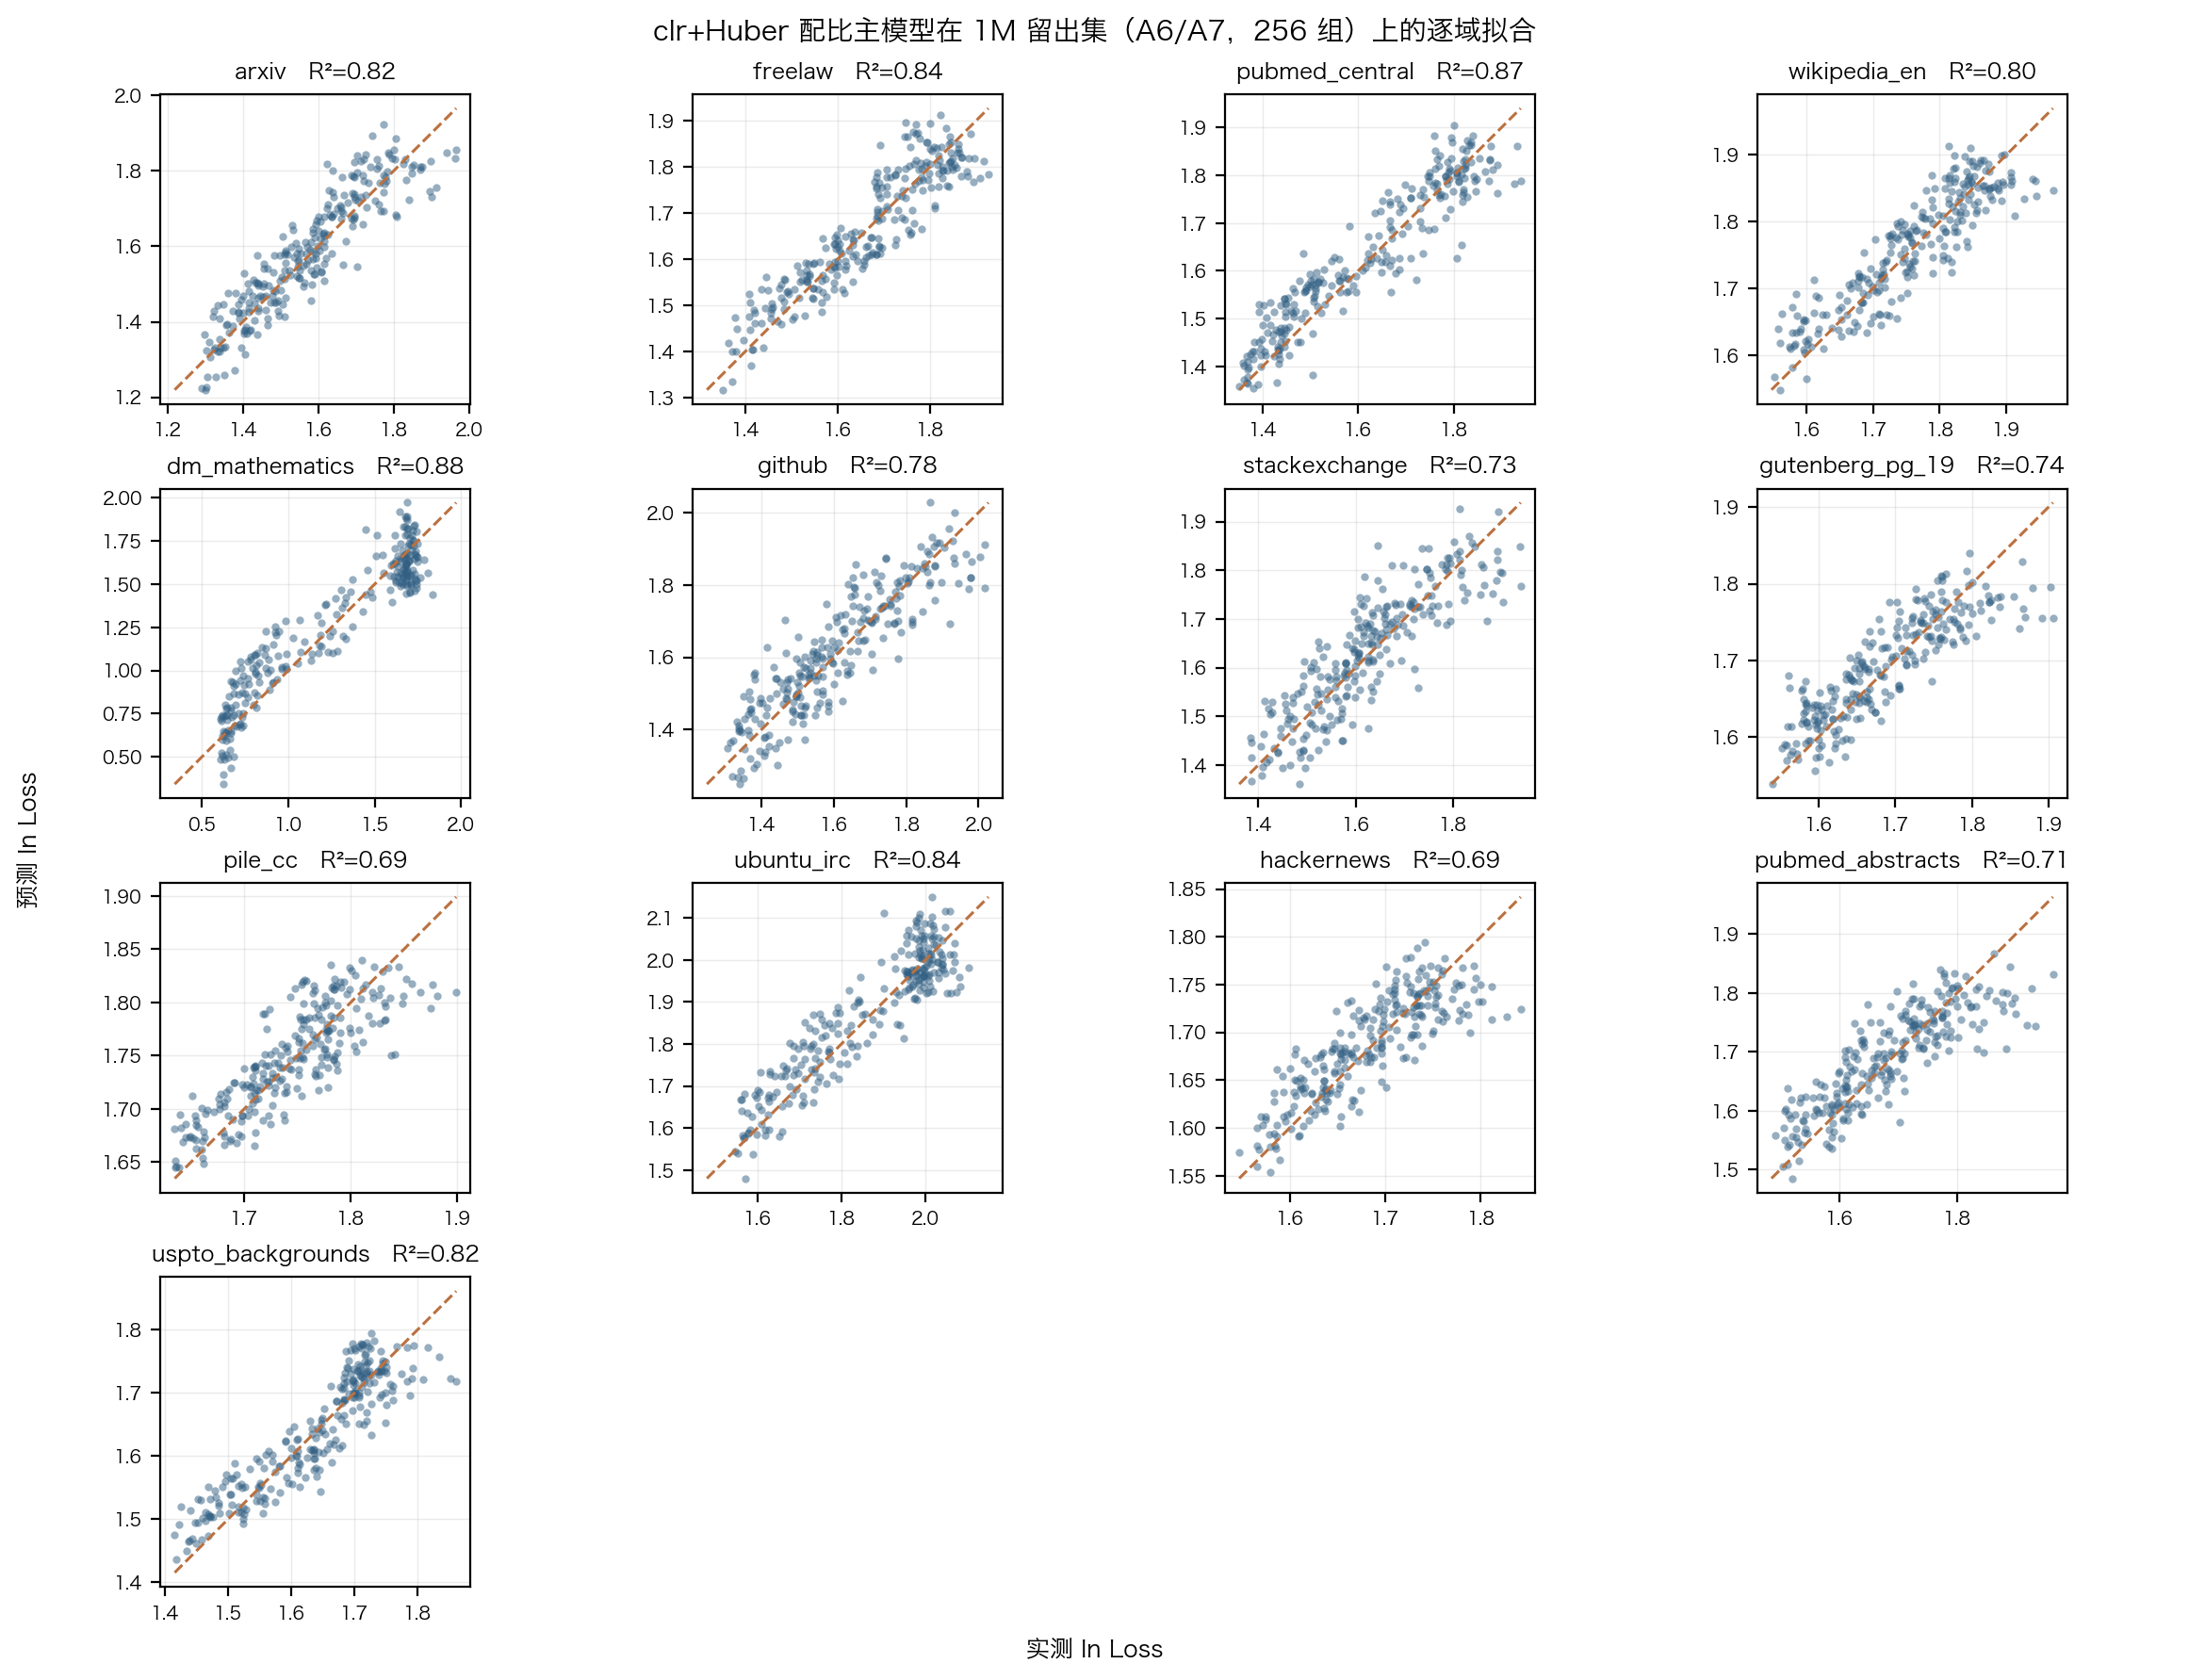
\includegraphics[width=\textwidth]{figs/q1_F5_mixture_fit.png}
\caption{配比主模型在 1M 留出集上的逐域预测与实测对数交叉熵（对角线为完全一致，子图标注对数空间 $R^2$）}
\label{fig:F5_mixture_fit}
\end{figure}

在线性模型的均匀配比处将系数投影到单纯形切空间，得到 $17\times13$ 迁移矩阵 $T_{iv}=17(\beta_{vi}-\bar\beta_v)$。图~\ref{fig:F5_transfer_matrix} 的主对角元均为负，表示在该局部位置提高某训练域份额时，其同名验证域的预测损失倾向下降；这是局部关联，不是因果效应。另加入质量交互项后，仅 6/13 个验证域的 bootstrap 区间不含零且方向不一，说明 $Q_i$ 无法代替配比实验来推断各域的训练边际价值。

\begin{figure}[H]
\centering
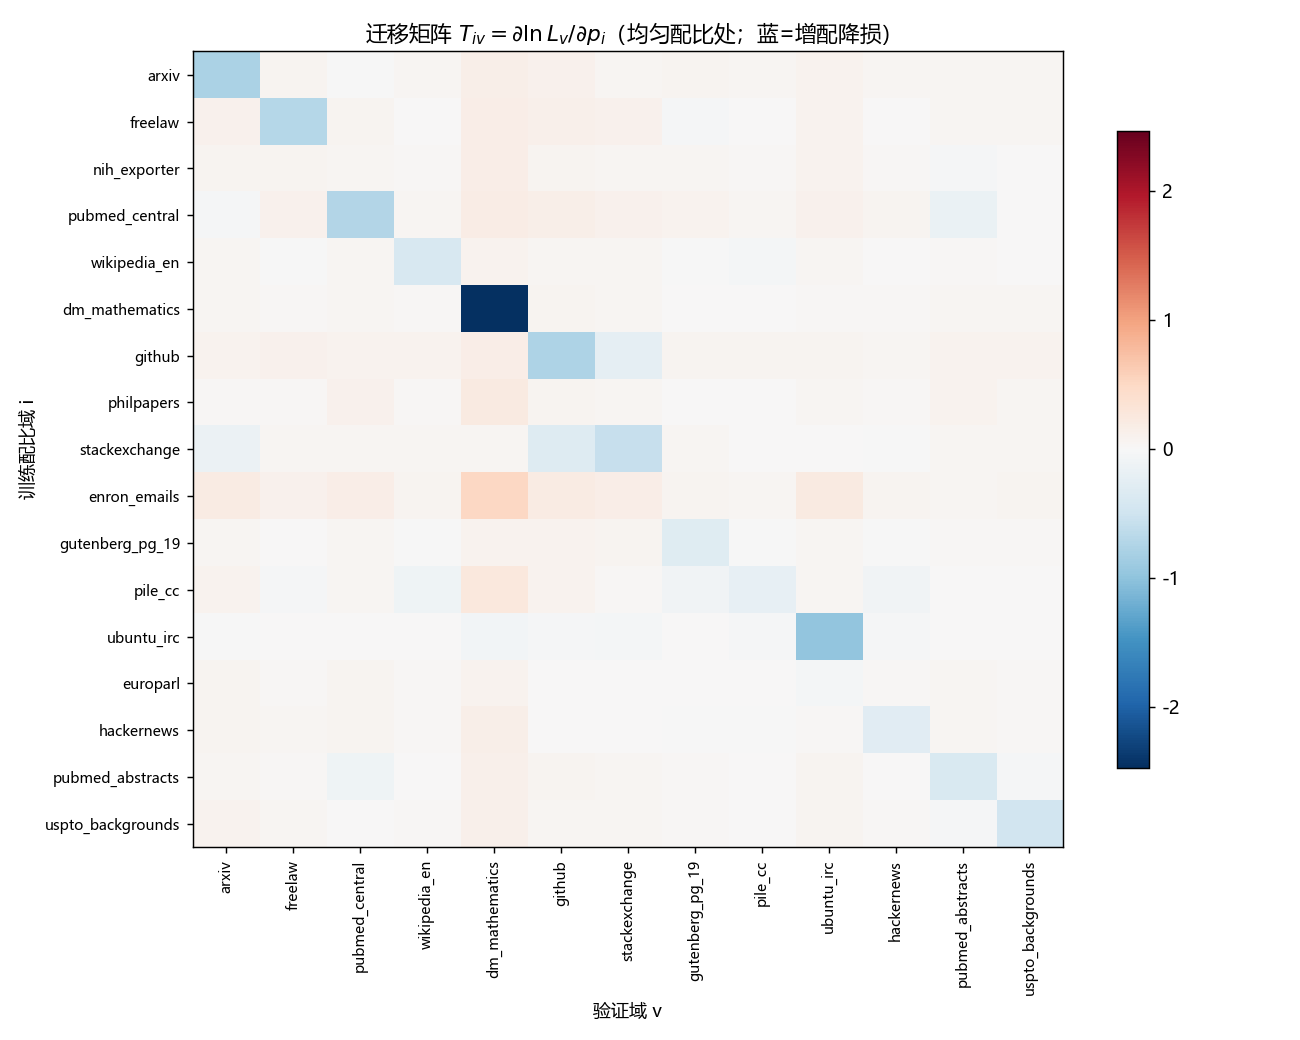
\includegraphics[width=0.92\textwidth]{figs/q1_F5_transfer_matrix.png}
\caption{$17\times13$ 迁移矩阵：各验证域对训练域份额的局部敏感度}
\label{fig:F5_transfer_matrix}
\end{figure}

\subsubsection{跨尺度检验与尺度修正}
\label{sec:q1_scale}

\paragraph{跨规模问题}式~\eqref{eq:q1_clr} 的系数来自百万参数模型的配比实验。把这一模型原样用于 6000 万和 10 亿参数模型时，需要分别检查两件事：它能否排出较优配比，以及它预测的交叉熵数值是否接近实测。后者存在明显的整体偏移，因此保留百万参数模型的配比系数，记 $g_v(\bp)=\boldsymbol\beta_v^{\rm 1M}\cdot\operatorname{clr}(\bp)$、$t=\ln(N/10^6)$，用下式修正不同参数规模下的预测：
\begin{equation}
\label{eq:q1_scale}
\ln L_v(\bp,N)=\underbrace{b_v^{\rm 1M}+\rho_v t}_{\text{截距漂移}}+\underbrace{s(N)}_{\text{效应缩放}}\,g_v(\bp),\qquad
s(N)=\left(\frac{N}{10^6}\right)^{-\lambda}\ \text{（本文采用）},\quad 1+\kappa t\ \text{（对照）}.
\end{equation}
式中 $\rho_v t$ 调整各验证域交叉熵的整体水平，$s(N)$ 调整配比变化的影响幅度。$b_v^{\rm 1M}$ 与 $s(10^6)=1$ 来自 A4/A5；A8/A9（6000 万参数）仅用于确定 13 个 $\rho_v$ 与共同缩放参数（幂律 $\lambda=-\ln s(60{\rm M})/t_{60}$），A10/A11（10 亿参数，各 64 组）不参与估计，只作独立检验。幂律形式在查看 10 亿参数结果前预先登记：它保持 $s(N)>0$ 并随规模单调衰减；对照的 $1+\kappa t$ 在很大规模下可能变负。

\paragraph{配比优劣顺序}图~\ref{fig:F6_mixture_order_agreement} 比较同一批配比在“预测的 13 个验证域等权交叉熵”和实测交叉熵下的优劣次序；Spearman 相关系数越接近 1，越能把低损失配比排在前面，但它不衡量交叉熵数值预测是否准确。线性模型在 1M 留出、60M、1B 上分别为 $0.523/0.467/0.677$；GBDT 为 $0.942/0.905/0.761$。树模型在三个规模上排序更一致，但到 1B 已下降，且该档只有 64 组配比。

\begin{figure}[H]
\centering
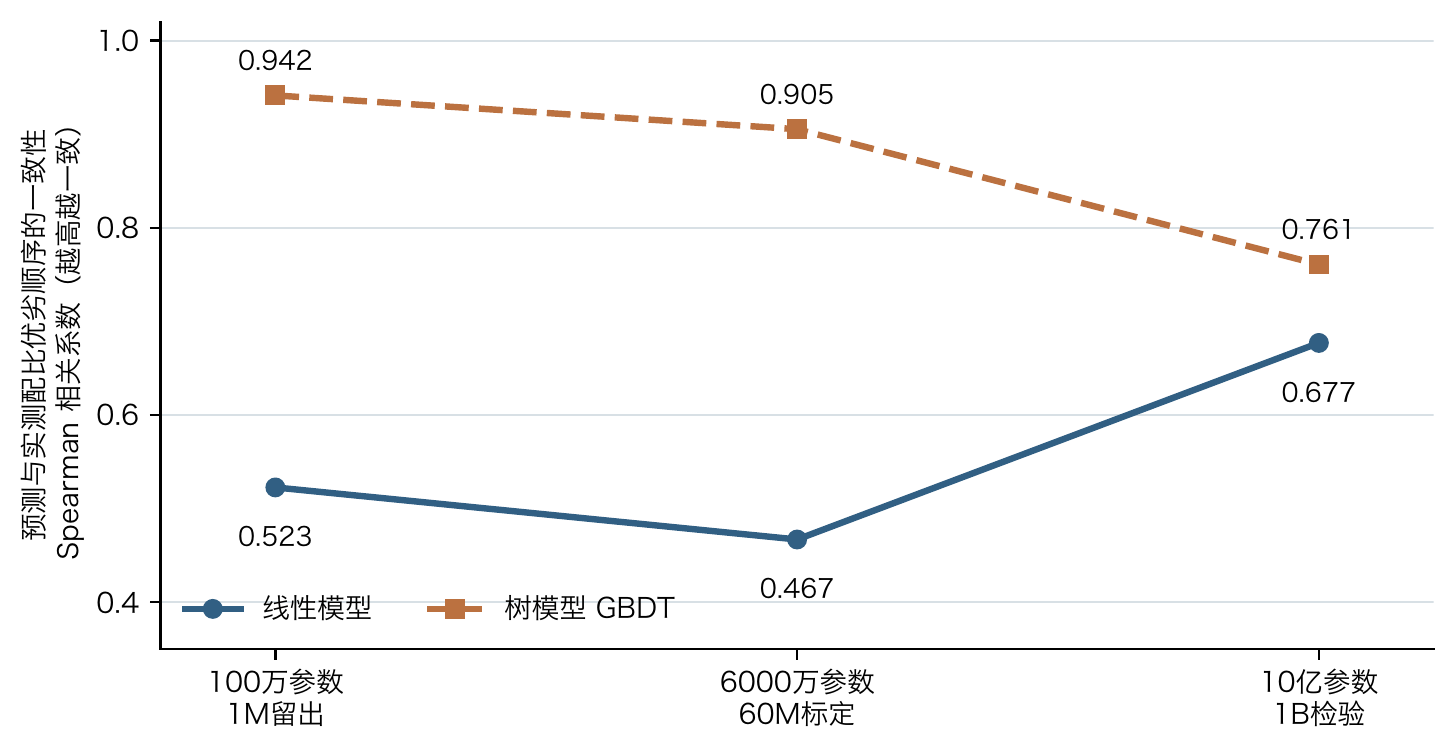
\includegraphics[width=0.88\textwidth]{figs/q1_F6_mixture_order_agreement.png}
\caption{在百万参数模型实验上训练的领域配比模型：预测与实测配比优劣顺序的一致性}
\label{fig:F6_mixture_order_agreement}
\end{figure}

\paragraph{交叉熵数值}图~\ref{fig:F6_scale_loss_comparison} 的每根柱表示该规模全部配比、13 个验证域的平均交叉熵，数值越低越好。6000 万参数是修正参数的标定集：实测均值 $3.82$，直接沿用百万参数模型预测为 $5.31$，修正后为 $3.81$，其接近实测属于同集标定效果。10 亿参数才是独立检验：实测 $2.23$，直接预测 $5.18$，修正后仍为 $3.00$。因此修正大幅缩小了水平误差，却未充分捕捉交叉熵随模型增大的下降幅度；A12–A15 的非观测估算不纳入该图。

\begin{figure}[H]
\centering
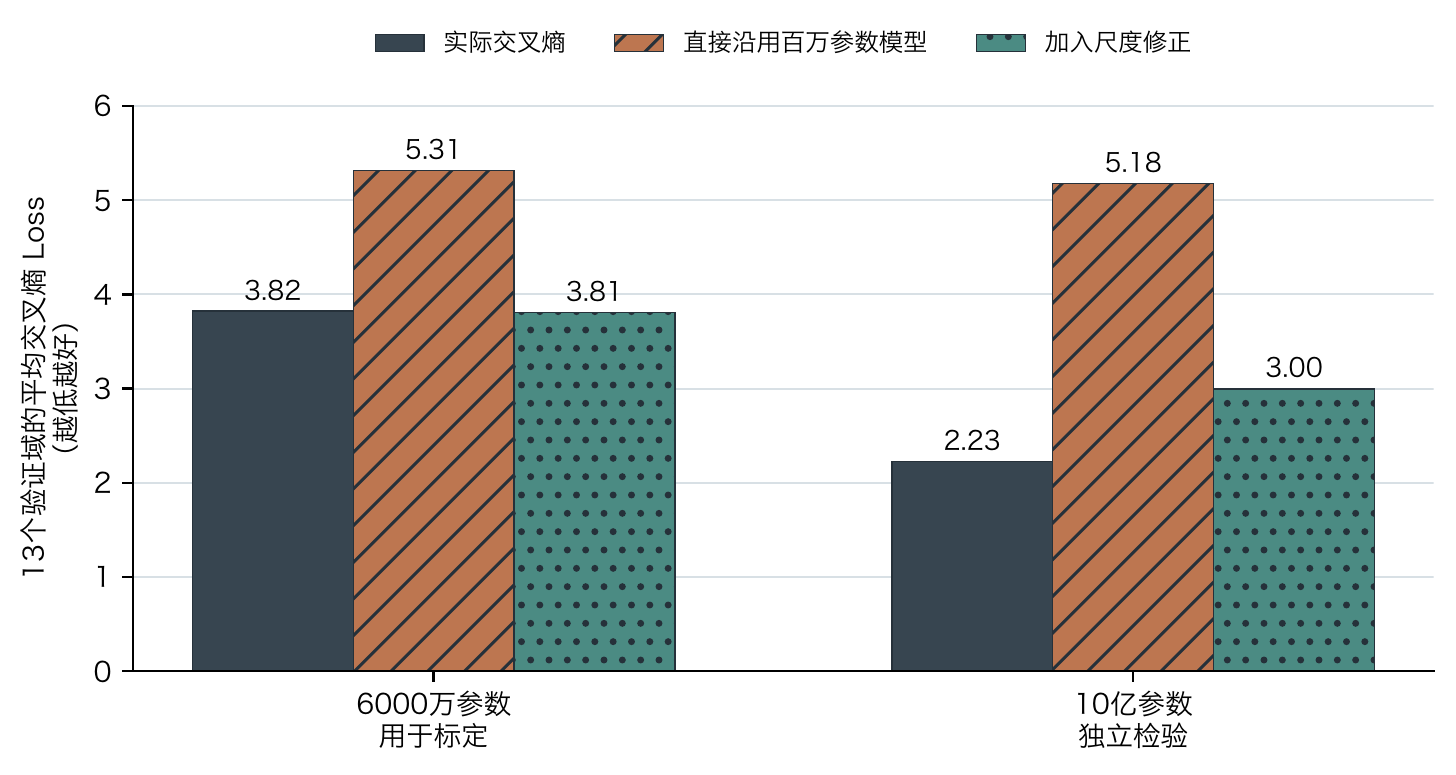
\includegraphics[width=0.88\textwidth]{figs/q1_F6_scale_loss_comparison.png}
\caption{6000 万参数标定集与 10 亿参数独立检验集的平均交叉熵：实测、直接预测与尺度修正后预测}
\label{fig:F6_scale_loss_comparison}
\end{figure}

\paragraph{逐组误差}表~\ref{tab:q1scale1b} 的 MAE 是每组配比、每个验证域预测交叉熵与实测值的绝对差再取平均，区别于图~\ref{fig:F6_scale_loss_comparison} 中仅比较总体均值。表中“未修正”即直接沿用百万参数模型；“同集拟合”使用了 10 亿参数数据估计参数，只作误差下界参照。独立检验上，修正使逐域 MAE 由 $2.9525$ 降至约 $0.77$（约 $74\%$），等权目标的排序相关由 $0.677$ 升至约 $0.713$，但逐域 $R^2$ 仍为负，说明数值外推仍不理想。

\begin{table}[H]
\centering\footnotesize
\caption{10 亿参数模型上的独立检验结果（A10/A11，各 64 组；数据源 \texttt{T6\_scale\_correction.csv}）}
\label{tab:q1scale1b}
\begin{tabularx}{\textwidth}{@{}p{2.8cm} r r r r r@{}}
\toprule
预测方法 & 逐域 MAE 均值 & 目标 MAE & 逐域 $R^2$ 均值 & 目标 Spearman & 平均预测 Loss \\
\midrule
未修正 & 2.9525 & 2.9525 & $-604.7$ & 0.677 & 5.178 \\
仅修正截距 & \textbf{0.7699} & \textbf{0.7684} & $-33.4$ & 0.712 & 2.994 \\
截距＋幂律缩放 & 0.7711 & 0.7708 & $-35.2$ & 0.713 & 2.996 \\
截距＋线性缩放 & 0.7714 & 0.7712 & $-35.3$ & 0.713 & 2.997 \\
同集拟合（参照） & 0.0819 & 0.0287 & 0.624 & 0.702 & 2.222 \\
\bottomrule
\end{tabularx}
\end{table}

\paragraph{形式选择与误差含义}按预先登记的规则，幂律修正在 10 亿参数上的逐域 MAE 为 $0.7711$，略低于对数线性对照的 $0.7714$，两者的等权目标排序相关同为 $0.7127$，故采用幂律形式。但 $0.0003$ 的误差差距远小于 64 组样本的抽样波动，选择主要基于幂律保持正值且随规模衰减的结构性质，不能把这点差距解释为预测精度的可靠提升。

修正后的主要误差来自水平外推：观测交叉熵每增加一单位 $\ln N$ 的平均下降幅度，从 1M$\to$60M 的约 $0.08$ 增至 60M$\to$1B 的约 $0.19$，两档数据无法识别这一曲率。配比效应的幂律外推为 $0.858$，而在 10 亿参数数据上同集拟合得到 $0.612$，表明配比影响实际衰减得更快；后者只用于定位偏差，不回填预测模型。同一函数形式直接在 10 亿参数上拟合时 MAE 约 $0.08$，它仅是同集误差下界，不代表跨规模预测能力。

\paragraph{校准接口与外推反例}固定百万参数模型系数计算的汇总校准斜率，在 1M 训练/留出/60M/1B 上为 $1.004/0.995/0.913/0.612$（\texttt{P1\_scale\_calibration.csv}）。前两档接近 1，后两档下降，表示训练配比差异对交叉熵的影响随模型规模增大而减弱；该斜率不是质量准确率。A12–A15 是估算/外推表而非观测，其同配比目标排序相关为 $-0.532/-0.588$，与 1M$\to$60M 实测的逐域 Spearman 均不低于 $0.98$ 不一致，因此仅作为更大规模外推风险的反例。

\subsubsection{推荐配比与接口输出}
\label{sec:q1_pstar}

\paragraph{候选最优配比}以 A4 平均配比为中心、用四档浓度 Dirichlet 生成 99,996 个候选。本文在线性模型的\textbf{信赖域}内选取推荐配比：候选 clr 向量到 A4 训练配比的马氏距离（协方差加 $10^{-3}I$ 岭）不超过训练配比自身距离的 $95\%$ 分位，且每域份额不超过 A4 该域最大值。信赖域内分别按 13 域等权损失与 pile\_cc 单域损失，取预测最优的前 100 个份额平均，得到 \texttt{p\_star\_eqweight}、\texttt{p\_star\_pilecc}；GBDT 在同一信赖域内另选 \texttt{p\_star\_gbdt} 作稳健对照。信赖域阈值取 clr 马氏距离 $21.85$，保留 46,168/99,996 个候选；不加信赖域时，线性模型会在远离训练分布的组合上给出不可信的低损失，故信赖域是必要的防外推设置。

\paragraph{推荐配比结果}表~\ref{tab:q1pstar} 给出各候选配比的对照。推荐配比 $\bp^*$ 使预测等权损失降到 $4.875$，较均匀配比（$5.385$）下降 $9.47\%$；线性模型与 GBDT 选出的配比高度一致（全变差距离 $0.0344$，即两配比各分量绝对差之和的一半；改用 GBDT 交叉评估线性模型所选配比，收益同为 $9.47\%$）。固定 $\bp^*$ 的 bootstrap 收益中位数为 $9.54\%$、$95\%$ 区间 $[7.82\%,11.16\%]$，每次重选结果与推荐配比的全变差中位数仅 $0.019$（图~\ref{fig:F7_p_star}）。该收益是 1M 代理模型内的预测差异，用于在真实训练前指导配比选择。

\begin{table}[H]
\centering\footnotesize
\caption{候选配比对照（数据源：\texttt{T7\_pstar\_benchmark.csv}、\texttt{P1\_p\_star.csv}）}
\label{tab:q1pstar}
\begin{tabularx}{\textwidth}{@{}p{2.7cm} r r r r r r@{}}
\toprule
配比 & \makecell{线性预测\\等权 Loss} & \makecell{GBDT 预测\\等权 Loss} & \makecell{线性\\评估收益} & \makecell{GBDT\\交叉评估收益} & 马氏距离 & $\bar Q$ \\
\midrule
$\bp^*$ 等权（线性，本文采用） & 4.875 & 4.901 & 9.47\% & 9.47\% & 13.9 & 0.66241 \\
$\bp^*$ GBDT 对照 & 4.927 & 4.811 & 8.51\% & 11.12\% & 10.4 & 0.66297 \\
$\bp^*$ pile\_cc（线性） & 5.074 & 4.963 & 5.77\% & 8.31\% & 4.0 & 0.66393 \\
训练配比均值 & 5.198 & 5.177 & 3.48\% & 4.36\% & 0.5 & 0.66399 \\
均匀配比 & 5.385 & 5.413 & 0 & 0 & 2.7 & 0.66065 \\
\bottomrule
\end{tabularx}
\end{table}

\begin{figure}[H]
\centering
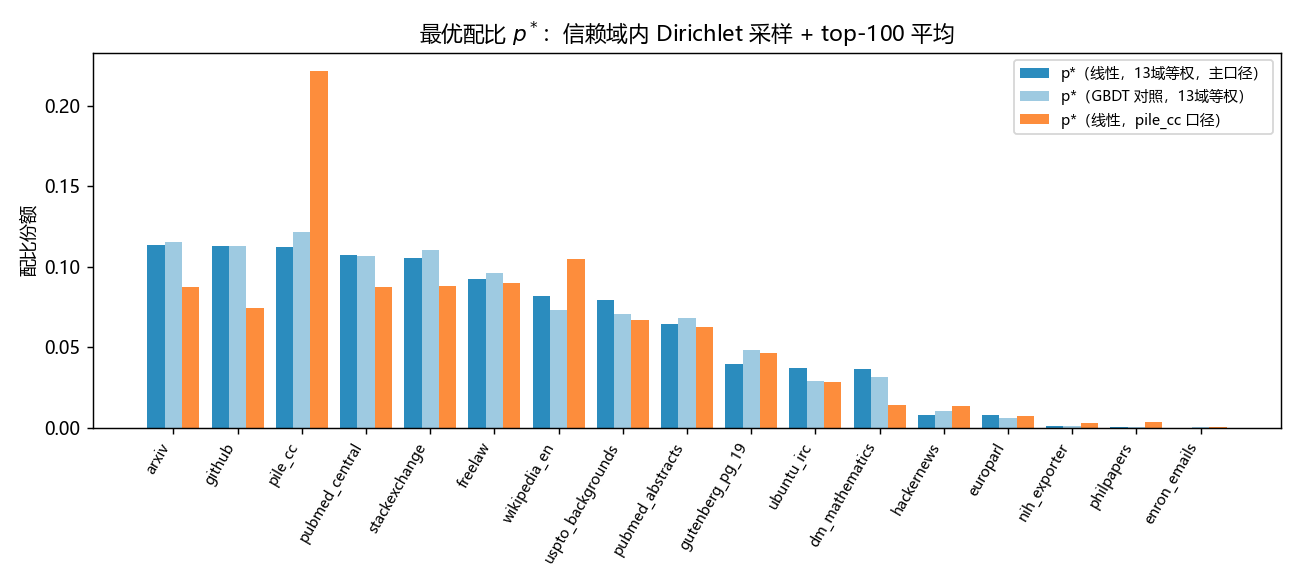
\includegraphics[width=\textwidth]{figs/q1_F7_p_star.png}
\caption{信赖域内候选配比分布与推荐配比、均匀配比位置}
\label{fig:F7_p_star}
\end{figure}

\paragraph{质量与训练边际价值的关系}17 域质量分与训练边际价值的 Spearman 仅为 $-0.211$（图~\ref{fig:F7_quality_vs_value}）：质量高的域其训练边际价值未必高，单凭质量分无法替代配比实验。推荐配比 $\bp^*$ 的配比加权质量 $\bar Q(\bp^*)\approx0.6624$，训练配比均值处为 $0.6640$、均匀配比处为 $0.6606$（\texttt{P1\_summary.json}）。

\begin{figure}[H]
\centering
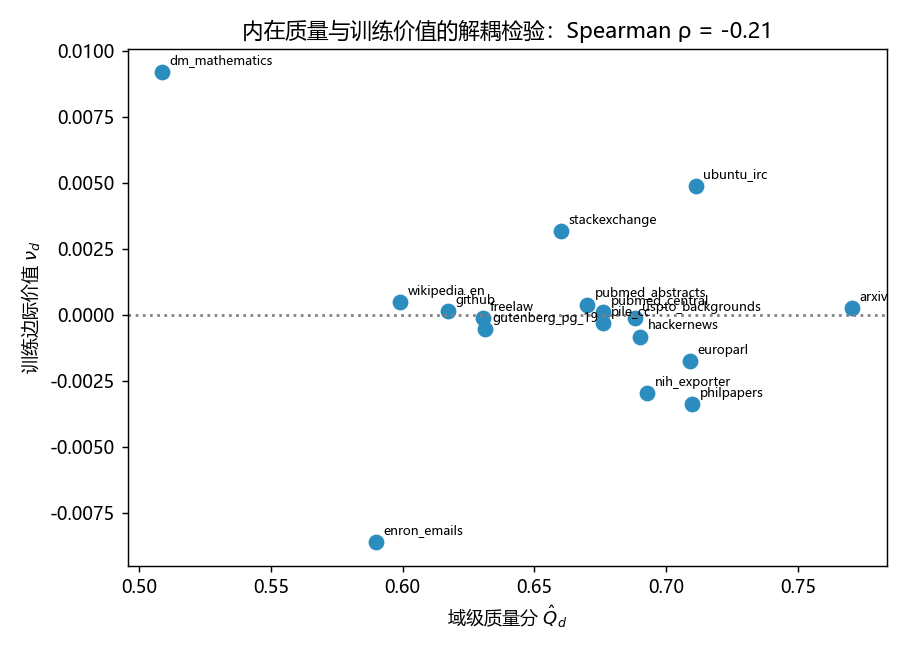
\includegraphics[width=0.78\textwidth]{figs/q1_F7_quality_vs_value.png}
\caption{17 域质量分与训练边际价值的散点关系}
\label{fig:F7_quality_vs_value}
\end{figure}

\clearpage
\subsection{本章小结}
\label{sec:q1_summary}

本章以 CRITIC 加权 Huber 模型量化文档质量，以六来源分歧模型识别指标间相反评价，再通过领域桥接和 clr+Huber 配比模型把质量与训练配比接入验证交叉熵。表~\ref{tab:q1_summary_metrics} 汇总各环节最能说明结果及其边界的指标。

\begin{table}[H]
\centering\small
\caption{问题一的关键结果及其实际含义}
\label{tab:q1_summary_metrics}
\begin{tabularx}{\textwidth}{@{}p{2.0cm} >{\raggedright\arraybackslash}p{5.2cm} >{\raggedright\arraybackslash}X@{}}
\toprule
环节 & 关键指标 & 含义与边界 \\
\midrule
质量评价 & A1 arxiv、wikipedia 的域级 $Q$ 中位数分别为 $0.7707$、$0.5991$ & 在同一评分规则下两域有明显差异；无人工真值，不能解释为质量准确率 \\
冲突识别 & RPS 组内 Kendall $W=0.140$；$69.45\%$ 的 A1 文档在该组同时出现高低两端指标 & 同一规则来源内部也会给出相反相对评价，不能仅用来源中位数概括全部指标 \\
领域桥接 & 分层五折 $R^2=0.4106$ & 规则特征能保留部分质量排序；11 个 inferred 域的分数仍受模型与跨域偏差影响 \\
配比选择 & 推荐配比在 1M 代理模型中预测等权交叉熵降低 $9.47\%$（bootstrap $95\%$ 区间 $[7.82\%,11.16\%]$） & 这是实验覆盖区域内的模型预测收益，不是重新训练模型后的实测改善 \\
跨规模检验 & 10 亿参数的逐域 MAE 由 $2.9525$ 降至 $0.7711$；平均预测交叉熵仍为约 $3.00$，实测约 $2.23$ & 尺度修正减小了误差，但绝对损失水平的外推仍有明显偏差 \\
\bottomrule
\end{tabularx}
\end{table}

领域质量 $Q_i$、推荐配比 $\bp^*$、配比—损失系数与尺度校准信息经 P1 接口传入问题二，为质量与配比进入广义标度律提供输入；问题三据此研究算力预算下的模型和语料配置，问题四再检验损失预测与 Benchmark 表现的联系。桥接估计及跨规模外推的局限需要在后续结论中继续保留。
